\chapter{Технологический раздел}
\label{cha:impl}

В данном разделе представлены средства, которые будут использованы для реализации программного комплекса. Описаны детали реализации программных компонентов, которые составляют основу системы, а также процесс обучения разрабатываемой нейронной сети. 

\section{Выбор средств разработки}

\subsection{Выбор языка программирования}

Python широко известен как один из самых популярных языков программирования для машинного обучения. Язык программирования предлагает большое множество библиотек, специально разработанных для задач данного вида. Эти средства разработки предоставляют комплексные инструменты для манипулирования данными, предварительной обработки, разработки и оценки моделей. Наличие готовых библиотек снижает необходимость реализации сложных алгоритмов с нуля, позволяя ускорить разработку и эксперименты. Python легко интегрируется с другими языками и инструментами, что делает его гибким выбором для проектов машинного обучения. Он легко взаимодействует с C/C++, обеспечивая эффективные вычисления, когда производительность имеет решающее значение.

Таким образом, простота, удобство чтения, обширная библиотека, универсальность, сильная поддержка сообщества и широкое распространение в промышленности и научных кругах сделали Python языком выбора для многих специалистов в области машинного обучения. Ввиду описанных ранее преимуществ для реализации программного обеспечения был выбран язык программирования Python последней актуальной стабильной версии 3.11 \cite{python}.

\subsection{Выбор библиотеки для машинного обучения}

PyTorch и TensorFlow --- две популярных библиотеки глубокого обучения, которые широко используются для разработки и обучения моделей \cite{pytorch} \cite{tensorflow}. В таблице \ref{tabular:deeplearing_frameworks} рассмотрены некоторые особенности данных инструментов разработки. 

\begin{table}[h!]
	\centering
    \captionsetup{justification=raggedleft,singlelinecheck=false}
	\caption{\label{tabular:deeplearing_frameworks} Сравнительная таблица библиотек для машинного обучения}
	\begin{tabular}{|p{4 cm}|p{5.5 cm}|p{5.5 cm}|}
		\cline{1-3}
		\textbf{Особенность}  & \textbf{PyTorch} & \textbf{TensorFlow} \\ \cline{1-3}
        Динамический вычислительный граф & PyTorch использует динамический вычислительный граф, что позволяет упростить отладку и повысить гибкость построения модели. & TensorFlow использует статический вычислительный граф, который предоставляет возможности для оптимизации, но может быть менее интуитивным и более сложным для динамических моделей. \\ \cline{1-3}
        Исследования и создание прототипов & PyTorch широко распространен в исследовательском сообществе благодаря своей гибкости, простоте экспериментов и сильной поддержке динамических архитектур нейронных сетей.	& TensorFlow также используется для исследований, но PyTorch часто предпочитают для быстрого создания прототипов и быстрых итераций.\\ \cline{1-3}
        Сообщество и ресурсы & PyTorch имеет быстрорастущее и активное сообщество с большим количеством руководств, примеров и исследовательских работ. В нем создана среда для совместной работы, которая поощряет обмен опытом и исследования. & TensorFlow имеет большое и устоявшееся сообщество с широким распространением в отрасли. Он пользуется поддержкой Google и предлагает широкий спектр ресурсов и предварительно обученных моделей. \\ \cline{1-3}
        Сообщество & PyTorch имеет развитую экосистему сообщества, которая включает новые архитектуры, функции потерь и предварительно обученные модели. Это способствует инновациям и позволяет быстро внедрять передовые методы. &	TensorFlow также имеет широкую экосистему, но вклад сообщества PyTorch был особенно заметен в последние годы. \\ \cline{1-3}
	\end{tabular}%
\end{table}

Для реализации описанного метода фильтрации малоразмерных шумов будет использоваться PyTorch ввиду своих преимуществ над TensorFlow.

\subsection{Выбор среды разработки}

Visual Studio Code (VS Code) --- это популярный редактор исходного кода, разработанный компанией Microsoft \cite{vscode}. Он является бесплатным, с открытым исходным кодом и доступен для Windows, macOS и Linux. Некоторые ключевые особенности и функциональные возможности Visual Studio Code описаны далее:
\begin{itemize}
    \item доступность для различных операционных систем позволяет разработчикам использовать его на предпочитаемой платформе;
    \item поддержка расширений, позволяющая разработчикам настраивать и расширять функциональность редактора;
    \item возможность использования интегрированного терминала устраняет необходимость переключаться между редактором и внешним интерфейсом командной строки, разработчики могут выполнять команды и сценарии непосредственно в редакторе;
    \item поддержка системы контроля версий Git, способствует легкому версионированию изменений разрабатываемого программного продукта, удобный интерфейс упрощает процесс фиксации изменений, ветвления, слияния и разрешения конфликтов;
    \item поддержка инструментов отладки для различных языков программирования;
    \item функционал гибкого редактирования внешнего вида редактора обеспечивает возможность изменять настройки в соответствии с индивидуальными предпочтениями;
    \item VS Code предлагает функцию совместной работы нескольких разработчиков в режиме реального времени, которая позволяет им совместно использовать рабочее пространство, редактировать код и сеансы отладки.
\end{itemize}

\subsection{Обучение нейронной сети}

Для обучения нейронной сети в качестве графического ускорителя был задействован NVIDIA RTX 3070 с общим объемом памяти 8 Гб. 

Количество эпох --- 50. На рисунке \ref{fig:loss_graph} описан график зависимости величины функции потерь от количества эпох. Следует отметить, что на выбранном наборе данных обучение более чем на 25--30 эпох не имеет большого смысла.

\begin{figure}[h!btp]
	\centering
	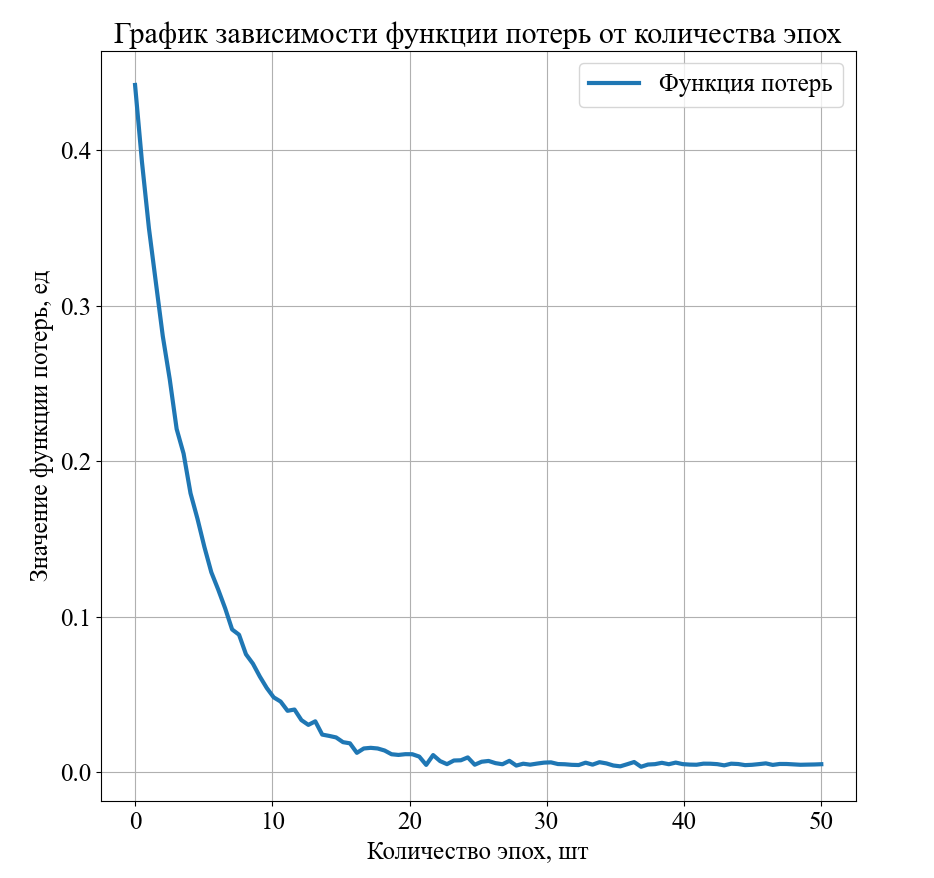
\includegraphics[scale=0.65]{inc/implementation/loss_graph.png}
	\caption{График зависимости функции потерь от количества эпох}
	\label{fig:loss_graph}	
\end{figure}

\section{Формат входных и выходных данных}

\textbf{Входные данные}:
\begin{itemize}
    \item путь до изображения с шумами;
    \item путь для сохранения результатов работы;
    \item (опционально) путь до изображения без шумов.
\end{itemize}

\textbf{Выходные данные}:
\begin{itemize}
    \item изображение, очищенное от шумов --- используется формат PNG без сжатия;
    \item (опционально) текстовый документ с метриками эффективности разработанного метода.
\end{itemize}

\section{Структура разработанного программного комплекса}

Разработанный программный комплекс состоит из 5 модулей, взаимодействие которых представлено в виде схемы на рисунке \ref{fig:prog_struct}.

\begin{figure}[h!btp]
	\centering
	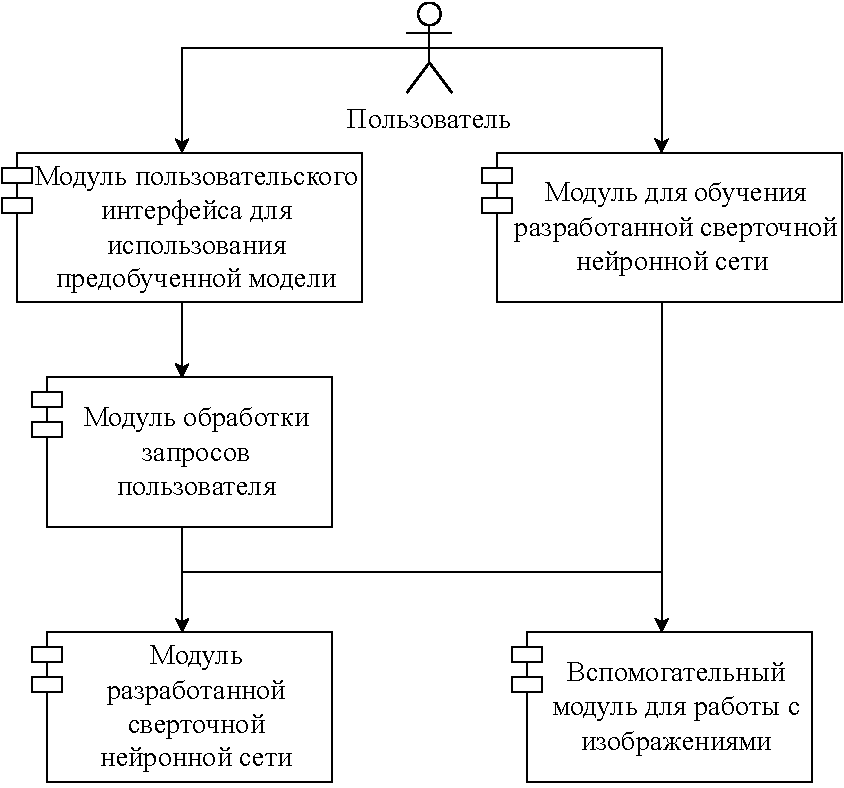
\includegraphics[]{inc/design/prog_struct.pdf}
	\caption{Структура ПО}
	\label{fig:prog_struct}	
\end{figure}

\section{Демонстрация работы программы}

Для взаимодействия пользователя с программным комплексом был реализован соответствующий интерфейс (см. рисунок \ref{fig:interface}) Путем по умолчанию является директория \textit{out} в папке программного модуля интерфейса.

\begin{figure}[h!btp]
	\centering
	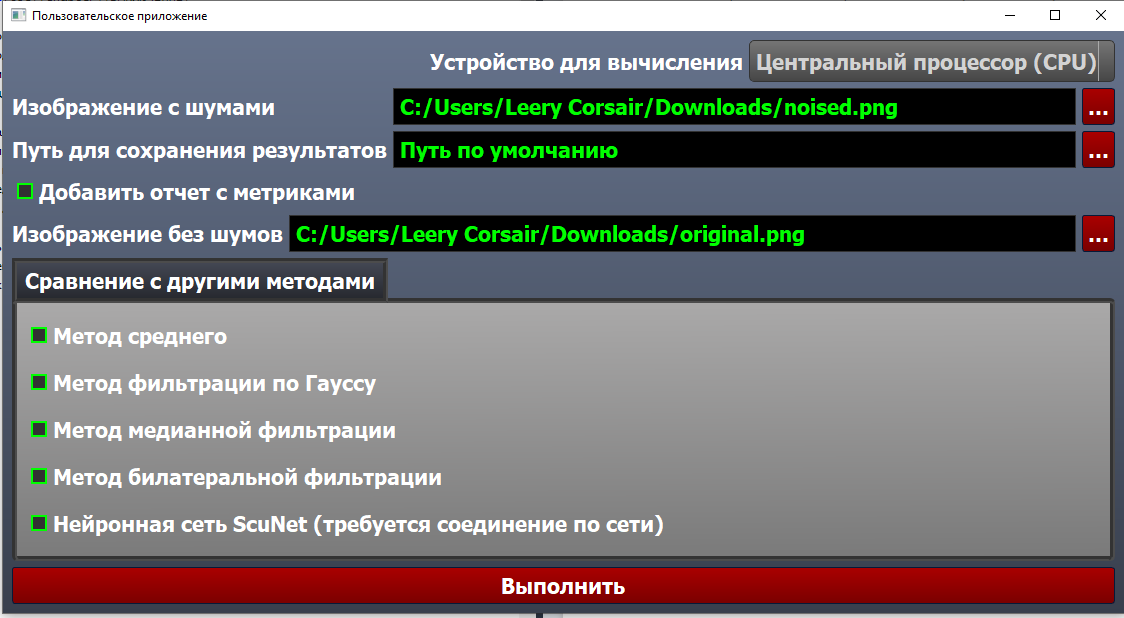
\includegraphics[scale = 0.5]{inc/demo/interface.png}
	\caption{Пользовательский интерфейс}
	\label{fig:interface}	
\end{figure}

На рисунке \ref{fig:demo} представлен пример работы программного комплекса.

\begin{figure}[h!]
  \centering
  \begin{tabular}{cc}
    \begin{subfigure}{0.45\textwidth}
      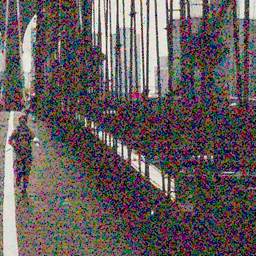
\includegraphics[width=\linewidth]{inc/demo/noised.png}
      \caption{Изображение с шумами}
    \end{subfigure} &
    \begin{subfigure}{0.45\textwidth}
      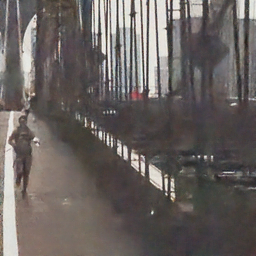
\includegraphics[width=\linewidth]{inc/demo/denoised_mycnn.png}
      \caption{Изображение без шумов}
    \end{subfigure} \\
  \end{tabular}
  \caption{Пример работы программы}
  \label{fig:demo}
\end{figure}

\newpage

\section{Выводы}

В данном разделе были описаны выбранные средства разработки, реализован программный комплекс, описан формат входных и выходных данных, а также продемонстрирована работы программы.